\section{The Political Philosophy of Confucianism}

\begin{quotex}
\textbf{OKAWA Shumei} (1886-1957) was a Japanese religionist and class-A war criminal. In 1942, after the bombing of Pearl Harbor, he wrote an introduction to Islam and translated a book about the ``perennial wisdom". He was arrested by the Americans for his political leanings and faced certain execution. On the first day of the Tokyo Trials, upon entering the courtroom he yelled randomly in German and slapped Prime Minister Tojo on the head, and was shortly found to be insane. While in the mental hospital, he made the first Japanese translation of the Qu'ran.

In this essay, which first appeared in the magazine\emph{ East Asia }in October 1930, Okawa advocates for a radical break with Western political thought by reviving and revitalizing Confucian order.

\end{quotex}
To aspire to Confucianism is without a doubt to make clear the Tao. And since the Tao is nothing if not a principle for individual life, Confucianism is an attempt to expound how men might live a righteous life. Now, a righteous life is a principle that realizes the correct relation between what we call ``I" and what we call ``not I". Confucianism divides what is ``not I" into the Three Powers, Heaven, Earth, and Man. This is the Tao of Confucianism. To be precise, Confucianism is the principle that realizes the proper relations between Heaven, Earth, and Man. In China, the scholars considered least worthy were thought of as ``lacking knowledge even of the Three Powers". When the English poet Wordsworth versifies on the necessity of holding a proper idea of God, Nature, and Man, it corresponds to this precisely.

\begin{wrapfigure}{rt}{.3\textwidth}
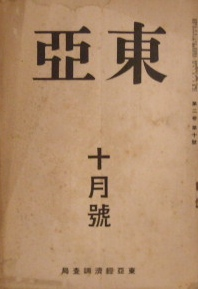
\includegraphics[scale=.5]{a20130223ThePoliticalPhilosophyofConfucianism-img001.jpg} 
\end{wrapfigure}

Now, Confucianism teaches that he who accords to Nature knoweth the Way. Mencius says that ``you must possess the five virtues yourself and extinguish your selfish nature", and this means the same thing. The autonomy of morality, which Kant outlined so carefully with his utterly precise logic, was not a unique discovery of the German philosophers. The Confucians rapidly grasped this truth based on their depth of experience. For example, Mencius' Four Sprouts are none other than a study of the foundations of human morality. What he calls a ``Sprout" is a ``natural foundation" from which morality can be grown. And so, in Confucianism, to work for ethical completeness is called development, or self-growth, or self-discipline. This capacity is inherent in oneself–he who possesses infinite possibilities for future action must start with an education in what is good. Therefore, the Tao as it pertains to Heaven, Earth, and Man first and foremost is something that should be realized through growing the natural foundations of morality in the self.

What is Heaven? Heaven is the origin of our existence. Most directly, this is our parents, and above them is our kin and ancestors. The origin of our ancestors is in the race, and the origin of that is in the universe. The correct relation to hold towards Heaven, that is to say, ``religion", is called in Confucianism Honor. This means growing and refining our essential human feelings of reverence and respect.

What is Earth? It is Nature as regarded by the mind. The most personal encounter we have with this is through our physical bodies, as well as the accompanying feelings of desire in our minds, as well as the external changes that these desires demand. The correct relation to hold towards Earth, meaning first the establishment of control over one's mind with regards to nature, and second the unification of one's attitudes, which may narrowly be called ``morality", is called in Confucianism Right. This means disciplining and training the essential human sense of shame, so that we will face towards Heaven unashamed and have good expectations for our life on Earth.

What is Man? Men are the individuals of good character whom you value equally with yourself. A well-bred man reasons with logic and acts with morality. Using logic, he understands the limitless possibilities of the complete knowledge of the universe, and thus is endowed with infinite possibility to realize in our lives, according to our intentions, the meaning of all things that it is possible to know. This personal limitlessness is called in Confucianism ``natural intellect, natural ability". Therefore, the proper relationship towards Man is to constantly develop the capacities of our natural intellect and ability, to our mutual benefit. Saying that this is realized through a purification of our natural tendency for sympathy and sentiment, Confucianism calls this Virtue. However, the collective effort to develop many intellects and abilities according to the parts of each and every life of many human beings in community is usually called politics. That is to say, the term politics is nothing other than an attempt to objectivize, or systematize Virtue.

Confucianism is therefore a Tradition that clarifies the three interests of religion, morality, and politics. Rather than breaking up these three ideas into separate fields of specialization, it understands them to interoperate as a single whole, and endeavors to eluciate the ``Tao" as a principle for all human life which contains all three. This is a point which has caused much outside confusion about the nature of Confucianism. One [Western Orientalist] will claim that Confucianism is a moral teaching, another will claim it chiefly conveys information about government, while still another lists it among the world's religions, but all their interpretation began from this source. For example, one Prof. Douglas calls Confucius' teaching nothing more than ``a plain, matter-of-fact system of morality". But Confucianism is not a religion in the Western conception of the thing, nor is it ethics or political science. Confucianism is not a single one of those, but is indeed all of them at once. Recognizing this as an internal structure, we can resolve the external confusion: this is a Tradition which we will understand nothing of from a Western perspective.\footnote{A postwar revision, and further thoughts on the concept of ``religion", can be found on my website: \url{http://avery.morrow.name/blog/2013/02/the-tao-of-the-east-and-the-last-samurais-testament/} }

\begin{quotex}
Here, \textbf{OKAWA Shumei} begins to make his departure from the basic principles of Western political thought obvious, deploying a slightly Hobbesian character from the 3rd century B.C., and demonstrating his Confucian orthodoxy. It is interesting to consider this contrast of rules vs. rulers in the modern cases of businesses, schools, etc.

\end{quotex}
The political thought of Confucianism is built on top of this fundamental spirit. Accordingly, most orthodox Confucianists could not be made to target politics as a thing standing alone and separated from religion and morality. The personal training for politicians, given names like ``study of ethical use of authority" and ``way to a virtuous nation", was never a thing separated [from the basic texts and principles]. According to Confucianism, as politics is the embodiment or systematization of Virtue, so the most essential basic requirement of the politician is to amass much virtue in their hearts. So most Confucian political works are expositions of knowledge intended for the ruler or politician. That is, to explain to the ruler the correct attitude for his heart, and how to attain virtue and compassion in his heart, is the basic method of Confucian political science.

For example, the Han \emph{Treatise on Punishment and Law} states, ``An ancient saying has it that even if the whole room has been eating and drinking, if there is one person crying to herself in the corner, no one in the room can enjoy themselves. And for a ruler, just like the case of that room, if even one person in his realm is treated unfairly, one's heart takes pity." An edict of Emperor Zhang of Han states, ``The sovereign must treat the people as if he were their father or mother, answering hardships with love, teaching loyalty and virtue, and administering appropriate punishment." Throughout the \emph{Shi Jing}, the ruler is portrayed as the mother or father of the people.

Indeed, as a consequence of understanding politics as the embodiment of Virtue in this way, the political ideal of Confucianism can be summarized in a phrase as ``domestic tranquility". Domestic tranquility means that for all of the people that exist in a nation, throughout their lives, negatively speaking they meet with no obstacle, or positively speaking, they are able to fulfill their respective functions. Nevertheless, regardless of the institution or organization, the expectation of true domestic tranquility does not mean that it is rigidly enclosed by [bureaucratic] considerations. At the top of Xunzi's thesis on sovereignty, he uses the phrase, ``\textbf{Rulers, Not Rules}``. And this phrase is the single clearest declaration of Confucian philosophy as it relates to systems and organizations, meaning that the aim of politics is not the \emph{rules}, but the \emph{character of the politicians}. Indeed, Xunzi's full statement is as follows:

\begin{quotationx}
Not a country in disorder, but a leader in disorder; not rules of order, but rulers in order. The methods of the archer Yi are not lost, yet such an archer does not appear generation after generation. The laws of King Yu of Xia still exist, yet the Xia could not continue their rule. Thus, laws cannot stand alone. Categories cannot apply themselves. If there are good men then the nation will survive. If there are no good men then it will be lost. Laws are the sprouts of order, and the man of virtue is the field in which that order grows. If men were virtuous enough we could even do without laws, but if no man is virtuous, no laws will suffice to save us, and we will fall into disorder. One who can simply count off the laws without knowing the Right behind them, no matter how learned you might call him, if he is given authority disorder will result. Therefore, a good king goes swiftly in search of good men, while a bad king seeks out power.

You ask how to rule a nation. You should first ask how to discipline yourself, before you can run a nation. The sovereign rules, and with his right rule comes right views. The sovereign is a bathtub, and his people are like the water. Water follows the shape of the tub. If he is a round tub, they will be round, and if he is a square tub, they will be square. It does not matter if it is the sovereign's edicts or his mere whims. King Zhuang of Chu preferred slender bodies, so there was starvation at court. If you must ask how to discipline yourself, you do not yet know how to rule your nation.
\end{quotationx}

Mencius means the same thing when he says frankly that ``without men of virtue, there can be no rule", and a famous chapter from Confucius' \emph{Doctrine of the Mean} goes, ``The government of Wen and Wu is recorded on tablets. Let there be such men and the government will thrive; but without such men, the government decays. With men who heed the Tao, government flourishes, just as agriculture flourishes when the Tao of the Earth is heeded; indeed, government matures just as reeds shoot forth from the soil," expressing the same idea.

The theory being expounded in \emph{Doctrine of the Mean} is as follows. An ideal government existed in the time of Kings Wen and Wu, which can be verified through various documents. People like them can govern splendidly, but without people like them, good governments can crumble. If good people are promoted to government, it is like plants growing from rich soil, and the results will come quickly. The rise and fall of individual politicians has immediate consequences in politics, just as a sudden change in soil quality has an immediate influence on the plant. Regardless of political system, our politics depends on the character of the people in it. And the type of people who will be appointed depends solely on the character of the ruler. Moral principles must be protected to establish good character. And virtuous love must be cultivated to possess those moral principles.

\begin{quotex}
Translation notes: The term ``man of virtue" means an educated elite, and is similar to how Julius Evola employs the term ``Aryan".

The Confucius translation is adopted from several English sources, rather than Okawa's incomprehensible late medieval transliteration (which he re-translates in the next paragraph). The first fourth of the Xunzi translation, about the archers and the Xia, is derived from Kurtis Hagen, \emph{The Philosophy of Xunzi}, Open Court Press, 2007. The rest is original and somewhat loose, but I swear to God he really does say the sovereign is like a bathtub.

\end{quotex}

\hfill

\begin{quotex}
Now, \textbf{OKAWA Shumei} takes out the big guns, attacking the founder of Legalism as impeding the cultivation of virtue, and by implication Western political theories which aim for the same legalistic goal. What the reader might not realize is that in denouncing Han Fei, who lived in the 3rd century B.C. and had an influence on all Far Eastern political thought thereafter, Okawa is arguing for a return to a very ancient ideal indeed. When a group of ultra-nationalists tried to overthrow the constitutional monarchy of Japan in the name of direct Imperial rule, Okawa was sent to prison for five years for providing the theoretical principles for such a political concept.

\end{quotex}

This concept, the greatest conceivable system to realize human ideals in an actual nation, comes into obvious opposition with the political philosophy of the West, which attempts to induce people to march automatically, so to speak, towards progress and perfection. Western political thought, in the words of Xunzi, has ``rules, but no rulers"; that is to say, it values creating good ``laws" over creating good ``men". Even in China, some sages like Shen Dao, Yin Wen, and Han Fei value law over men in their writings. Han Fei, especially, fiercely attacks the idea of ``rulers without rules" in one of the chapters of his book, and devotes himself to organizational structure. What he claims is that waiting for a man of virtue to appear is like a hungry man refusing to eat for a fortnight while he waits for a prime rib to arrive; the poor soul will simply starve to death.

His argument goes like this: Even with a total disinterest in organizational structure, a nation can be ruled by the likes of an Emperor Yao. And even with the finest organizational structure, a nation ruled by a tyrant would quickly dissolve into chaos. But a great Emperor Yao or a tyrannical King Jie will appear only once in a thousand years. Most rulers are neither Yao nor Jie. To create a nation that can be ruled by ordinary rulers, we must create the appropriate institutions. Creating people rather than rules creates a nation that can only be ruled once in a millennia, while creating rules for people will make a nation that is only disrupted once in a millennia.

Han Fei declares this to be a truth that is difficult to deny, and indeed, if we place our faith completely in the personality of a ruler, the result will be as Han Fei describes. But in Confucianism, even if there have been some who put an undue emphasis on it, there has been no one who disputes the meaning and value of ``laws". Actually, in the \emph{Doctrine of the Mean}, the three major functions of the ruler are piety, governance, and intellect. Piety implies both religious courtesies and moral customs, while governance means legal and political systems, and intellect refers to literacy. Without grasping the aforementioned three things, one cannot be a ruler in either name or reality. Even the most earnest abstract desire for a ``domestic tranquility", without institutions in place to ensure true domestic tranquility, we would not expect anyone to call someone a real politician. Mencius says, ``Mere good intentions do not build a government, nor do mere laws." The ``mere" here means subjective, or abstract. Confucianism, therefore, does not at all ignore structure, but recognizes that spiritual development must be esteemed over mere structure.

The success of all systems is, without a doubt, the result of a success of the human spirit. Therefore the true meaning of a structure cannot be grasped by the people who join into that structure if they lack a spiritual foundation. It becomes accordingly difficult to maintain it effectively. A genius who knows all 3,000 rules of etiquette and 300 marks of majesty, if he fails to grasp the true meaning of piety, will simply fall into useless, machine-like imitations. And in order to grasp the true meaning of piety, we need true hearts and good faith. This is why Lu Jiuyuan said, ``If we fail to overcome our own selfishness, it will be difficult for us to know virtue. And without a full knowledge of virtue, we will know not what rules and regulations are for."

\begin{quotex}
I continue directly into the conclusion. Hopefully all the readers of this blog will be quite gratified to see this independent manifestation of the Traditional principles.

\end{quotex}


Now, in Confucianism, there is a strong emphasis on ``love for relatives", or ``veneration for noble deeds" as a principle for social life. In the \emph{Doctrine of the Mean}, Confucius teaches: ``The humanity of virtuous behavior is made evident in the case of love for relatives. The ability of righteousness to set things straight is made evident when we honor noble men. The decreasing measures of the love due to relatives, and the steps in the honor due to the worthy, are produced by the principle of propriety." The implication of this passage is, approximately, as follows. Virtuous love binds people together, and its most striking manifestation is in our natural affection for our parents and kin. In contrast, justice is a type of discrimination. Its most striking manifestation is when we naturally hold some sense of respect towards noble men, that is to say, those whose moral values tower above all of us.

Nevertheless, we do not love all of our relatives equally. Even if the original source of virtuous love is an indiscriminate, equal substance, it is utterly unforgivable for its manifestation to be uniform in nature. Our reverence towards ethical exemplars, too, is of the same nature. In the manifestation of virtuous love and reverence, the attempts to confer a correct order are the grounds that generate the various forms and systems of social life. It is an indispensable condition for a Confucian social order that social inequalities are generated from a correct moral foundation.

Both love for relatives and veneration for noble deeds are called much more simply ``filial piety" or ``respect for the elders". One of the first statements in the \emph{Analects} reads, ``A youth should be filial at home, and, when abroad, respectful to his elders." The model for household life necessitates recognizing the position of parents, and each sibling among the children disposes of his ``self" and faithfully works for the sake of his family and clan, continuously realizing an order of being. Honoring virtue, similarly, underlies the model for national life, and Confucius teaches that the exercise of authority both large and small necessitates a shared concept of virtue, which people must entrust to the statesmen, abandoning their ``self" interests and faithfully obeying the authority of the state.

Therefore, the duties of the men of noble birth in China were not rule of the country–personal oversight as administrators–in the usual sense, but were actually the promotion of able men to wield authority in roles both great and small. Therefore, it is said that ``if we hasten to get the right men, the self is checked and the nation is put in order, the merits are great and one's name is celebrated, and one is worthy of being called a sovereign. If we do not hasten to get the right men, but instead focus on getting the labor first, then people will work for their own purposes and divide the nation, merit is abandoned and one's name is besmirched, and the very soil and grain of the nation will certainly be endangered. The worthy sovereign seeks out the men and, having found them, may rest."

``If the people be led by laws, and uniformity sought to be given them by punishments, they will try to avoid the punishment, but have no sense of shame. If they be led by virtue, and uniformity sought to be given them by the rules of propriety, they will have the sense of shame, and moreover will become good." This is a famous saying of the \emph{Analects}, and a summary of the essential spirit of Confucian political philosophy. […] And there is one point on which Confucianists and Legalists agree. Namely: what constitutes an upright citizen, in other words the attempt to forge a tempered and cultivated political individual, is a separate matter from the legal system, in other words the attempt to establish a systematized nation-state. Again, in other words, while Legalism insists on the strictly impartial nature of legislation, Confucianism remains the first principle at the root of litigation [because the goodness of a person is based in Confucian values].

In this way the political doctrine of Confucianism is generally not called one of constitutionalism, but is rather rite-ism, and the relation between laws and rites is perfectly encapsulated by Liang Qichao, who said that ``laws treat the symptoms, but rites are preventative health." According to Confucian political science, the sole foundation of good government is indeed cultivation of culture and learning: ``right learning brings good customs, and good customs bring good government."

The political thought of Confucianism, as clearly indicated by all the histories, was never implemented closely in China. The finest implementation of it up until now was in our own nation's Tokugawa period. The shape of our nation in that era rivals and even exceeds that of China's Spring and Autumn period, showing that the political ability of the Japanese far outstrips that of Han Chinese. The China of the Spring and Autumn Period was not much different from the old shogunate in population, area, or feudal development. Accordingly, the political ideals of Confucius and Mencius, although meant for a united China, became much more relevant in our own country, and our political ability was not just a realization of those ideals but a superior realization to that of China.

Thus in the Tokugawa period, the ideal that made the sovereign parent to the nation became ingrained in the hearts of the provincial lords, and when one province achieved a temporary state of good leadership, other provinces felt a need to compete [as in sibling rivalry] and strained to achieve the same standard, creating a splendid government. That China later descended into pandemonium and confusion despite its cultivation of Confucianism is not due to any insufficiency in Confucianism itself, but the fault lies in the political incompetence of the Han.

\begin{quotex}
The pointedness of this last paragraph lies in the fact that Okawa has just made use of brilliant reformists like Liang Qichao (1873-1929), but unlike their Japanese counterparts, the Chinese reformists failed to rebuild and modernize China.

All credit for the production of this translation lies with the Okawa Shumei Study Group which made these materials available. All fault for the numerous translation errors and misrepresentations lies with me.

\end{quotex}


\flrightit{Posted on 2013-02-21 by Avery Morrow }

\begin{center}* * *\end{center}

\begin{footnotesize}\begin{sffamily}



\texttt{Lemonheadz on 2013-02-22 at 00:28 said: }

Did Okawa have any contact with Guénon or his school of thought?


\hfill

\texttt{Avery Morrow on 2013-02-22 at 00:35 said: }

Okawa unfortunately seems to have missed out on Guénon and his school. His leanings in that direction, though, are demonstrated by a book he translated for a man named Paul Antoine Richard, the husband of Sri Aurobindo's spiritual successor ``The Mother". Richard's book is indistinguishable from Aldous Huxley's The Perennial Philosophy which was written 2 or 3 years later. After long conversations with Richard, Okawa became a big fan of Sri Aurobindo despite a lack of thorough reading into his philosophy.


\hfill

\texttt{Jason-Adam on 2013-02-22 at 17:58 said: }

Honour also consists in admitting your sources. You don't learn from China and Korea and then take their women as your sex slaves and their men as forced labour. Japan behaved with great dishonour during WW2 and was punished by Heaven for it.

I strongly advise that in studying the Far Eastern form of the tradition, we should avoid the Japanese derivative forms and look to the roots in China and Korea…..

For the record let me also say that the Koreans are a much stronger martial people than the Japs, they beat the French and Americans in the XIXth century and the Japs many times over the centuries, last time being WW2.

I am presently preparing to be initiated into a Korean order…..


\hfill

\texttt{Avery Morrow on 2013-02-22 at 21:24 said: }

I can't really comment on your principle that the truthfulness of a text can be judged by the circumstances its author lived in, nor that military defeat is a sign of martial strength, but I feel obliged to at least correct your inaccurate claim of ``sex slavery"; not only was no slavery involved in Japan's military brothel system, but it was taken over by the Americans and used in the Korean War, and a similar system was set up by the Americans in Vietnam, purchasing women from impoverished Vietnamese families. Please see this academic summary of research into the subject.


\hfill

\texttt{Janus on 2013-02-23 at 17:37 said: }

I must disagree here…the extent to which a woman in poverty can really be said to be ``willing" in her prostitution is highly debatable. The amount of freedom she really had once in the hands of soldiers, Japanese or American, even more so.


\hfill

\texttt{Janus on 2013-02-23 at 17:42 said: }

The tripartite division of Confucianism presented here is interesting, but does it not focus more on the cult of the ancestors than the cult to Divinity? Or is this Divinity contained in the ``universe" which births the race, ancestors and parents?

The acknowledgement of Confucianism as an organic ``living" practice, rather than just a philosophy is essential and something I am glad to see here. The western insistence on dividing learning, work, life, religion, and so on is a major sign of its degeneration. His comment on the western perspective is spot on, although I must agree with doubts expressed about using the Japanese rather than original Chinese perspective, particularly one coming from the Imperial era of the 20th century rather than pre-Meiji Ishin.


\hfill

\texttt{Jason-Adam on 2013-02-23 at 17:57 said: }

It's a tricky matter. My grandfather was a rikuguntaisa in the Japanese army during the Greater East Asia War but after visiting Korea I feel as if I need to make penance for his misdeeds.


\hfill

\texttt{Avery Morrow on 2013-02-24 at 06:43 said: }

This is too late at this point, but I'm sorry for my rather accusatory and grumpy comment. I thought about it a lot today, and I am certain my attitude stems directly from reading too many high-tempered Internet arguments.


\hfill

\texttt{Jason-Adam on 2013-02-28 at 21:53 said: }

The author shows his racism by blaming the problems of China on racial defects and not on failures of character, failures that afflict men in all nation, and have made Japan a cultural and political colony of America since 1945.

In fact, China under the Qing dynasty was a quite stable and functional regime until the British imposed opium addiction on the Chinese people.

I see a contradiction in that the author praises Edo period Japan, which was a peaceful, feudal, and autarchical era yet he supported ultra-nationalism which was more like Fascism in supporting an expansionist centralised state under the dictatorial rule of the Mikado who was no longer the spiritual figurehead he was under the shogunate but an actual Bonaparte-type sovereign under this sytem (I'm thinking also of Ikkai Kitta)


\hfill

\texttt{Avery Morrow on 2013-02-28 at 22:01 said: }

You forget that China was not the only East Asian nation struggling with Western interference; Japan was also thrown into crisis by Western temporal power, and its response was quite different from China, while its blazing fast modernization and militarization was due in large part to the efforts of Emperor Meiji himself.

Okawa witnessed the failure of both China and Korea to adapt in his own lifetime, and the near subjugation of both nations by the West; he has ample reason for his patriotic attitude. I would wager that he is actually a more appealing figure than Evola, who discarded sentimental ties to family and nation.


\hfill

\texttt{Jason-Adam on 2013-03-01 at 18:01 said: }

Modernisation……that's the problem…….in order to fight the West, Japan became a western power. 

China and Korea failed, yes, though in the Korean case the failure is arguable as I can attest to the survival of Korean tradition through my own studies in that nation. But the failure is simply that of traditional falling to modern which is not a good thing in my book, as I'm a supporter of the old ways.

Asian patriotism like any patriotism is a good thing but not when it becomes a tool for colonialism – if Japan had led Asia against the West he'd have been heroic but instead the Japs decided to just enslave fellow Asians in Manchuria, Korea, and China.

PS – the US tried to open up Korea in 1866 the same way they did with Japan in 1853 but that time the Koreans won and the big noses came home dead…….

I prefer Evola's attitude of placing principles above false realities……he saw the true state of his Italy and did not fail to expose it…..


\hfill

\texttt{Avery Morrow on 2013-03-01 at 18:44 said: }

To try to drag the discussion back to the actual nature of this essay, I don't think Evola's political vision is that far from Okawa's, except that the situation in Italy ensured that Evola could never dream of implementing a Traditional government, whereas Okawa had many adepts hoping to do just that.


\hfill

\texttt{Jason-Adam on 2013-03-01 at 23:13 said: }

I hope I am discussing Okawa's essay here when I raise issue with the fact that he claims China never properly implemented Confucianism, I would like to know that if he is correct, then how would he describe the ruling ideology of the Chinese empire from the Han dynasty (200 BC) to the end of the Qing (1912 not counting its revival in Manchukuo, 1930s)?

The difference I am seeing between Okawa and Evola, correct me if I am in error, is that whereas Evola wanted the unification of Europe under a supranational Emperor that transcended nationalisms, Okawa believes Japanese nationalism can unify Asia under Japanese domination ?


\hfill

\texttt{Janus on 2013-03-02 at 00:31 said: }

Fascinating piece, though I must too express my disappointment at his ease in asserting that there was some racial flaw in the Han which caused the decline in China, especially when he mentions periods in Chinese history when righteous rulers came to power. 

I'm also glad to see that he discussed Legalism, the philosophy predominant in influence in China today, especially on the political stage, and that he can do so without quickly dismissing it. Political ideas and movements are revealed for what they are without men and women of quality making up the numbers: utopian ideals at most, and farces leading to tyranny at worst (see the Conservative revolutionaries, who allowed their ideas to be hijacked by those for whom Aryans were a mere biological race). It is essential to make good laws in the State, but even more to realize that they are there to craft good human beings. This is the most radical assertion one can make in the political and social realm, and a dangerous one which can lead to tyranny if there is no direct and positive correlation between position in the hierarchy and standard of character and accountability. 

I heard two quotes in a performance of the Trial of Socrates which I think beautifully encapsulates the Confucian view in a democratic context: ``In a democracy, you're only asked to do two things: obey the law, and try to change it if you think it's wrong." and ``You accepted the constraints of the law every time you accepted our protection and did not speak in the Assembly in order to craft the best laws possible." Without good and just men, there is no good and just order.


\hfill

\texttt{Avery Morrow on 2013-03-02 at 05:09 said: }

What was actually implemented from 200 BC to the 1930s was Legalism, which was argued in this essay to be a distortion of the original tradition. (In the same way that the Christian medieval world was a distortion of the Roman imperium? Maybe? Hmm.)

That's a great question. I honestly don't think Okawa had such a naively imperialist view, but his geopolitical analyses are yet on my to-read list, and if I translate anything else by him on Gornahoor I will mention what I learn.


\hfill

\texttt{Jason-Adam on 2013-03-02 at 17:32 said: }

@ Avery

It would be good to read more of Okawa's ideas, as the close relationship between geopolitics and tradition is something I feel Guenon and Evola did not see…………

It's very interesting, the subject of Legalism, I remember reading once someone tried to argue that Maoism is actually derivative of Han Fei Zi, it is true that to some degree Mao admired Qin Shi Huang, the persecutor of the Confucians…… 

In a western context, do you think Plato is closer to Confucius or Han Fei ? The fact that he wrote a book of Laws seems to indicate P. thought he could legislate for a state beyond the capabilities of individual men ?


\hfill

\texttt{Avery Morrow on 2013-03-02 at 18:35 said: }

Just as a particular example, I think Plato's belief in the communal upbringing of children puts him squarely on the side of a Legalist legislating morality. That's not to say this idea is horribly dangerous, since Israel's kibbutzim implemented something like it and did not end in disaster. Nor is Legalism anti-Traditional; the early modern period was full of such attempts to preserve exoteric manifestations by putting them into law.

But the Roman imperium was not characterized by a huge list of laws and a great bureaucracy maintaining them. People's instincts for things like raising their own families were considered to be basically good, and only needed cultivation through education. I think Okawa and Evola are both right to claim that in the ``world of Tradition", Law is only expressed through obedience to the Principles, which are self-explanatory and within every human heart.


\hfill

\texttt{Avery Morrow on 2013-03-02 at 23:28 said: }

One last note: if anyone would like to flesh out their knowledge of Xunzi I found a Ph.D. thesis which supports Okawa's thesis that Xunzi defended real Confucianism from Legalism, actually closely imitating the conclusion that Confucianism supports the concept of laws but Legalism turns this into an obsession.

http://scholarspace.manoa.hawaii.edu/handle/10125/3023

Excerpt: ``While Confucian constructivism can support a theory of universal human rights, if it is to remain Confucian, it would not emphasize this because Confucianism perceives reasons not to foster a strong rights culture. Rights are viewed as legalistic mechanisms which, if over-emphasized, can erode informal mechanisms such as Ii (ritual propriety), the maintenance of which is considered critical to maintaining a healthy society. Citing several passages from the Xunzi, along with other Confucian texts, Ch'ii T'ung-Tsu concludes: `Confucians firmly believed that … The order or disorder of a state … depends completely upon the maintenance or the decay of li' (Ch'u, p. 241). To the degree rights seem to undermine rites, they will likely continue to be resisted."


\hfill

\texttt{Jason-Adam on 2013-03-02 at 23:57 said: }

Avery, so in your view one can be a Confucian or a Legalist and still be Traditional ?

Would you define the Torah or the Shariah as versions of Legalist thought ?

I wonder if the purpose of Confucianism and Legalism are for different ages, the age of Yao and Shun compared to our time from a Hindu perspective is different points and the cycle and different styles of governance perhaps may be required ?


\hfill

\texttt{Avery Morrow on 2013-03-03 at 00:24 said: }

I would agree that Confucianism and Legalism are both Traditional and suited different ages, since this is grounded in historical fact as well. It's also obvious that rabbinic halakah did not exist when Israel was a kingdom (the Torah and Talmud are not solely legal texts). But shariah just as clearly comes from the ``seal of the Prophets" himself, befitting the 8th century AD.

This exchange has made me wonder much more seriously whether a ``return to Confucianism" would approximate a Protestant desire for the simplicity of the earliest sources without the awareness that we are living in a degenerate age. Evola, of course, would disagree, and there are plenty of medieval texts that assert that Confucius takes primacy over his commentators, but I would like to see what Schuon says on the matter.


\end{sffamily}\end{footnotesize}
